%角动量加法

考虑两个系统,总角动量分别为 $l_1$  和 $l_2$, 可能的状态分别为 $\ket{l_1, m_1}$, $\ket{l_2, m_2}$. 角动量算符分别为 $L_1^2$, $L_{1x}$, $L_{1y}$, $L_{1z}$, $L_2^2$, $L_{2x}$, $L_{2y}$, $L_{2z}$.  

现在定义总角动量算符
\begin{equation}
J^2 = (L_1 + L_2)^2 = (L_{1x} + L_{2x})^2 + (L_{1y} + L_{2y})^2 + (L_{1z} + L_{2z})^2
\end{equation}
\begin{equation}
J_z = L_{1z} + L_{2z}
\end{equation}
令量子数分别为 $J$  和 $M$.  所有新增的对易关系为
\begin{equation}
\comm*{J^2}{J_z} = \comm*{J^2}{L_1^2} = \comm*{J^2}{L_2^2} = 
\comm*{J_z}{L_{1z}} = \comm*{J_z}{L_{2z}} = 0
\end{equation}
若限制  $l_1$ 和 $l_2$ 为常数,原来和现在的 Complete Set of Commutable Operators (CSCO) 是
\begin{equation}
\{L_{1z}, L_{2z}\} \qquad \{J^2, J_z\}
\end{equation}
现在已知前一组的本征基底 $\ket{l_1, m_1} \ket{l_2, m_2}$,  要求后者的基底 $\ket{J, M}$.  首先由对易关系, $\ket{l_1, m_1} \ket{l_2, m_2}$ 已经是 $J_z$ 的本征矢,每个 $M$ 可以有一个子空间,维数 $N$ 是 $m_1 + m_2 = M$ 的不同组合数(\autoref{AMAdd_fig1}).当 $\abs{M} = l_1 + l_2$ 时 $N = 1$ (唯一的非简并情况), $\abs{M} = l_1 + l_2 - 1$ 时 $N = 2$, 以此类推(但注意 $m_1$, $m_2$ 不能超出范围)

\begin{figure}[ht]
\centering
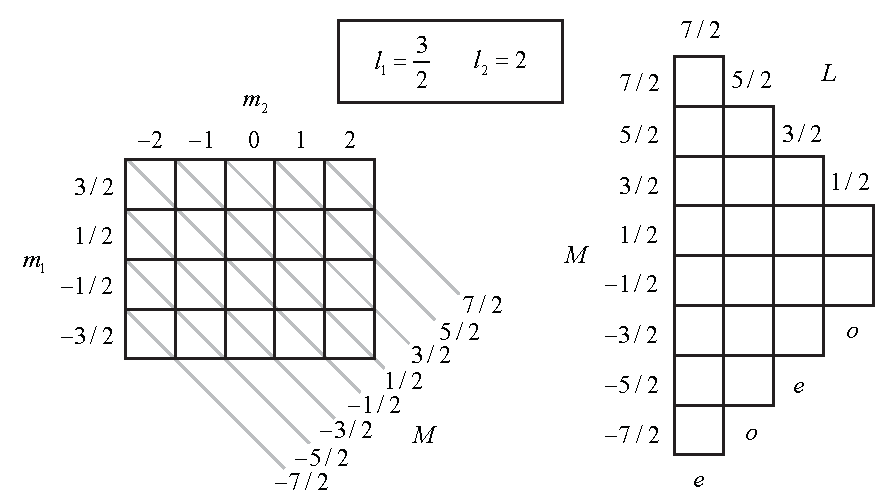
\includegraphics[width=10cm]{./figures/AMAdd1.pdf}
\caption{$\ket{l_1, m_1}$ 张成的 $2l_1+m_1$ 维空间和 $\ket{l_2, m_2}$ 张成的 $2l_2+m_2$ 维空间组成 $(2l_1+m_1)(2l_2+m_2)$ 维的外积空间, 这个空间也可以使用 $\ket{L, M}$ 作为基底, 且基底变换在每个 $M$ 子空间中独立进行} \label{AMAdd_fig1}
\end{figure}

\begin{equation}
N = \leftgroup{
&l_1 + l_2 + 1 - \abs{M} \quad (\abs{M} > \abs{l_1 - l_2})  \\
&\min\{l_1, l_2\} \quad \text{(其他)}
}\end{equation}
我们只需要在每个子空间 $M$ 中把 $J^2$  对角化即可.
\begin{equation}
J^2 = L_1^2 + L_2^2 + 2(L_{1x} L_{2x} + L_{1y} L_{2y} + L_{1z} L_{2z})
\end{equation}
其中只有 $L_{1x} L_{2x} + L_{1y} L_{2y}$  不是对角矩阵.利用升降算符表示
\begin{equation}
2 (L_{1x} L_{2x} + L_{1y} L_{2y} ) = L_{1+} L_{2-} + L_{1-} L_{2+}
\end{equation} 
\begin{equation}\ali{
&\bra{l_2, m'_2} \bra{l_1, m'_1} J^2 \ket{l_1, m_1} \ket{l_2, m_2}\\
&= \hbar ^2 \qty[ \ali{
&\delta_{m'_1, m_1} \delta_{m'_2, m_2} [l_1(l_1 + 1) + l_2(l_2 + 1) + 2 m_1 m_2]  \\
+ &\delta_{m'_1, m_1 + 1} \delta_{m'_2, m_2 - 1} \sqrt{l_1 (l_1 + 1) - m_1(m_1 + 1)} \sqrt{l_2 (l_2 + 1) - m_2(m_2 - 1)}\\
+ &\delta_{m'_1, m_1 - 1} \delta_{m'_2, m_2 + 1} \sqrt{l_1 (l_1 + 1) - m_1(m_1 - 1)} \sqrt{l_2 (l_2 + 1) - m_2(m_2 + 1)} }]
}\end{equation}
 
一般在一个 $M$ 空间中, $m_1$ 用降序排列, $m_2 = M - m_1$,  $m_1$ 的最大值为
\begin{equation}
\max \qty{m_1} = \leftgroup{
&l_1 \quad (M \geqslant l_1 - l_2)  \\
&l_2 + M \quad \text{(其他)} 
}\end{equation}
这样, $J^2$ 就是一个三对角矩阵,其本征矢矩阵就是从 $\ket{J, M}$ 表象到 $\ket{l_1, m_1} \ket{l_2, m_2}$ 表象的幺正变换矩阵 $\mat U_M$ ( $\ket{J,M}$ 的顺序取 $J$ 从大到小).矩阵的输入矢量可以用 $m_1$ 为角标,输出矢量可以用 $J$ 为角标.查 CG 表时, CG 系数通常以 $\mat U_M$ 矩阵的形式给出(如 Griffiths).可以证明, $\mat U_M$ 的 $N$ 个本征值为 $J(J + 1) \hbar ^2$,  其中 $J = l_1 + l_2, l_1 + l_2 - 1,\dots$ (共 $N$ 项%,不会证明
)(注意最小值大于但不一定等于 $\abs{M}$ ). $J$ 在所有子空间的最小值是 $\abs{l_1 - l_2}$ (当 $\abs{M} = \abs{l_1 - l_2}$ 时取得),所以 $J$ 在所有子空间的范围是
\begin{equation}
J = \abs{l_1 - l_2}, \dots, l_1 + l_2
\end{equation}
现在我们已经知道了每个子空间 $M$ 的变换,那么如何求总变换呢?先把总矩阵列表,行标题是所有的 $\ket{l_1, m_1} \ket{l_2, m_2}$, 列标题是所有的 $\ket{J, M}$, 对每个空间,找到对应的 $N$ 行和 $N$ 列,把 $N \times N$  的 $\mat U_M$ 矩阵照抄上去即可.


